\chapter{Variational Autoencoder Implementation Details} \label{ann:VAE}

In this annex, code implementation of the \ac{VAE} is provided. The \ac{VAE} is a generative model that is specifically designed to learn latent representations of data and enable controlled generation. The following sections elucidate the \ac{VAE} model's structure and its training process.

\section{Model Implementation}

The subsequent Python code exemplifies the execution of the simple \ac{VAE} model.

\begin{lstlisting}[language=Python]
class VAE(nn.Module):
    # ... (class operations)

    def forward(self, x):
        x = x.float()

        y = self.encoder(x)

        mean = self.meaner(y)
        logvar = self.varer(y)

        z = self._sample(mean, logvar)

        decoded = self.decoder(z)
        return decoded, mean, logvar

    def _build_encoder(self):
        layers = []

        layers.append(nn.Conv1d(1, 32, kernel_size=9, stride=1, padding=4))
        layers.append(nn.BatchNorm1d(32))
        layers.append(nn.Tanh())
        layers.append(nn.MaxPool1d(kernel_size=2, stride=2))

        for i in range(self.convolutional_layers - 1):
            layer = nn.Conv1d(2**i*32, 2**(i+1)*32,
                              kernel_size=9, stride=1, padding=4)
            layers.append(layer)
            layers.append(nn.BatchNorm1d(2**(i+1)*32))
            layers.append(nn.Tanh())

            layers.append(nn.MaxPool1d(kernel_size=2, stride=2))

        mean_layer = nn.Sequential(
            nn.AdaptiveAvgPool1d(1),
            nn.Flatten(),
            nn.Linear(2**(self.convolutional_layers-1)*32, self.latent_dim)
        )

        var_layer = nn.Sequential(
            nn.AdaptiveAvgPool1d(1),
            nn.Flatten(),
            nn.Linear(2**(self.convolutional_layers-1)*32, self.latent_dim)
        )

        return nn.Sequential(*layers), mean_layer, var_layer

    def _build_decoder(self):
        layers = []

        layers.append(
            nn.Linear(self.latent_dim, 2**(self.convolutional_layers-1)
                      * 32 * (self.input_size // 2**self.convolutional_layers))
        )

        layers.append(
            nn.Unflatten(1, (2**(self.convolutional_layers-1)*32,
                         self.input_size // 2**self.convolutional_layers))
        )

        for i in range(self.convolutional_layers - 2, -1, -1):
            layers.append(nn.Upsample(scale_factor=2))
            layers.append(nn.ConvTranspose1d(2**(i+1)*32, 2**i *
                                             32, kernel_size=9, stride=1, padding=4))
            layers.append(nn.BatchNorm1d(2**i*32))
            layers.append(nn.Tanh())

        layers.append(nn.Upsample(scale_factor=2))
        layers.append(nn.ConvTranspose1d(
            32, 1, kernel_size=9, stride=1, padding=4))
        layers.append(nn.BatchNorm1d(1))
        layers.append(nn.Tanh())

        return nn.Sequential(*layers)

    def _sample(self, mean, logvar):
        std = torch.exp(0.5 * logvar)
        eps = torch.randn_like(std)
        return eps * std + mean

    def loss_function(self, recon_x, x, mean, logvar):
        recon_x = torch.clamp(recon_x, 0, 1) # normalize output
        x = torch.clamp(x, 0, 1) # normalize input
        BCE = F.binary_cross_entropy(recon_x, x, reduction='sum')
        KLD = -0.5 * torch.sum(1 + logvar - mean.pow(2) - logvar.exp())

        return BCE + KLD
\end{lstlisting}

The \ac{VAE} model comprises an encoder, a bottleneck layer, and a decoder. The encoder analyzes the input data to extract significant characteristics, whereas the decoder produces reconstructions from covert representations. The latent space is sampled by employing mean and variance parameters from the encoder.

\section{Training Process}

The \ac{VAE} is trained with the following code.

\begin{lstlisting}[language=Python]
def train_step(data_loader, model, optimizer):
    model.train()

    train_loss = 0

    for batch, (sample, label, _) in enumerate(data_loader):
        # ... (input preprocessing)

        recon_batch, mean, logvar = model(sample)
        loss = model.loss_function(recon_batch, sample, mean, logvar)

        optimizer.zero_grad()
        loss.backward()
        train_loss += loss.item()
        optimizer.step()

        # ... (display and memory management operations)

    train_loss /= len(data_loader.dataset)
    return train_loss


def test(data_loader, model, name):
    model.eval()

    test_loss = 0

    with torch.no_grad():
        for sample, label, _ in data_loader:
            # ... (input preprocessing)

            pred, mean, logvar = model(sample)
            loss = model.loss_function(pred, sample, mean, logvar)

            test_loss += loss

            # ... (display operations)

    test_loss /= len(data_loader)

    return test_loss

def run():
    epoch = 0

    # ... (display and early stopping initializations)

    while True: # actual code had early stopping checking
        # ... (display operations)
        train_loss = train_step(dataloader_train, model, optimizer)
        loss = test(dataloader_test, model, f"{CONV_LAYERS}_{epoch}")

        epoch += 1

    # ... (display and memory management operations)
\end{lstlisting}

The training process iteratively updates the model with data batches. In each training step, the model is optimized with a loss function that combines \ac{BCE} and \ac{KL} divergence terms. The function encourages the model to produce accurate reconstructions and learn a significant latent space.

\section{Results}

As an illustration of the \ac{VAE}'s potential, this section exhibits two images: one featuring an initial audio waveform and the other displaying its reconstructed version produced by the trained \ac{VAE}.

\begin{figure}[ht]
    \centering
    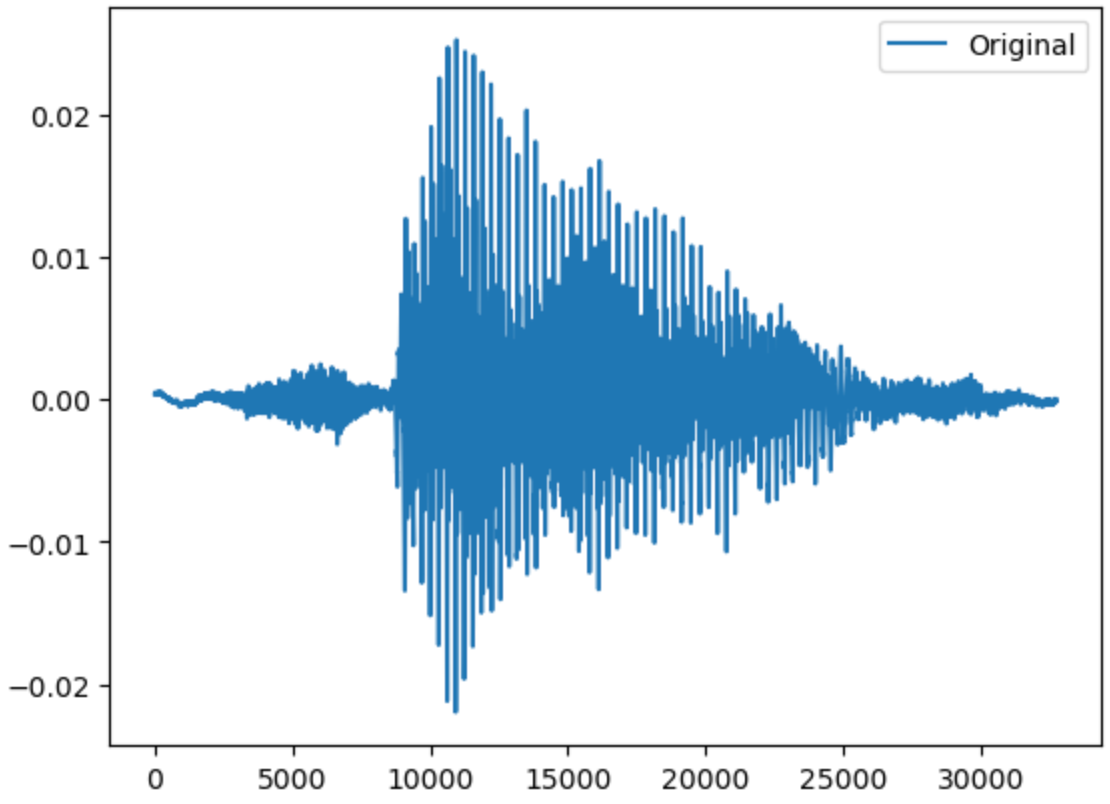
\includegraphics[width=0.7\linewidth]{figures/annexes/VAE/original.png}
    \caption{Original Sample}
\end{figure}

\begin{figure}[ht]
    \centering
    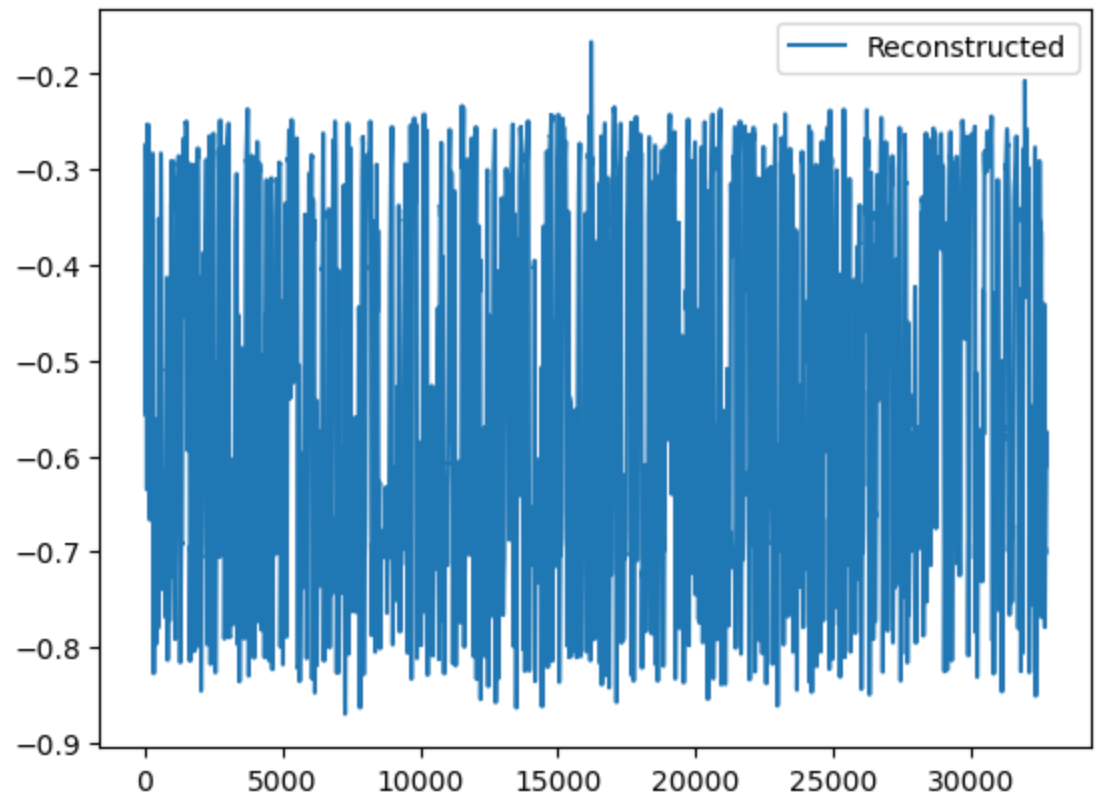
\includegraphics[width=0.7\linewidth]{figures/annexes/VAE/reconstructed.png}
    \caption{Reconstructed Sample}
\end{figure}

These images represent the best reconstruction achievable by the author, considering the hardware and time limitations.

\clearpage
